\chapter{Theory}
\label{chap:usage}

\section{What is a good image?}
\label{sec:setup}
Throughout this thesis we will mention the word quality several times. While some people already have a good understanding of what the word means, some confusion may arise. 

Within the standard image quality assessment field, quality´s definition is straight forward and is what most people think about when hearing the word. Ordinary people and people working with images will for the most part think about the image resolution as the most important characteristic that defines image quality. An excellent image of a face with this definition would have high resolution and sharp focus.   

However Mobai´s and our definition differs from the usual way image quality is defined. Our emphasis lies not with the image resolution itself, but rather how well the face is visible. There are several aspects that heavily affect the quality of facial images with respect to biometric systems performance. These aspects are presented and discussed in two important papers: 

\begin{itemize}
    \item ISO/IEC TR 29794-5:2010: Information technology — Biometric sample quality — Part 5: Face image data. \footnote{\url{https://www.iso.org/standard/50912.html}}
    \item ICAO Doc 9303 Part 3: Specifications Common to all MRTDs. \footnote{\url{https://www.icao.int/publications/Documents/9303_p3_cons_en.pdf}}
\end{itemize}

The quality specific aspects of facial images presented in the two standards are what defines the quality in our thesis. The different quality factors are:  

\begin{itemize}
    \item Image properties like the size of the image or its resolution.
    \item Image appearance characteristics like the exposure or noise.
    \item Scenery characteristics like lighting or background.
    \item Characteristics like the consistency between the skin colour on the image and the skin colour of the subject.
    \item Complete or partial face coverings.
    \begin{itemize}
        \item Glasses fully covering the eyes.
        \item Any type of head coverings.
    \end{itemize}
    \item The behaviour of the subject.
    \begin{itemize}
        \item Closed or open eyes.
        \item Closed or open mouth.
        \item Any kind of expression, e.g. smiling or neutral.
        \item Head pose, e.g. frontal or rotated in any direction.
    \end{itemize}
\end{itemize}

The above mentioned aspects all affect the quality of the facial image to some degree. What we consider an excellent facial image is similar to a standard passport image with the following characteristics: 
\begin{itemize}
    \item Open and visible eyes.
    \item No dark tinted glasses. 
    \item Neutral or little to none facial expression.
    \item Neutral head pose.
    \item No garments covering the face.
    \item Clean background.
    \item Neither too dark or too light.
    \item Photo taken neither too close or too far away.
    \item Face is centered.
\end{itemize}

The characteristics will affect the quality in a good or bad way. If all the bullet points above are true, the quality of the facial image is near perfect. An image of a half-covered or missing face will negatively affect the quality, even though the image resolution itself may be impeccable. 

\begin{figure}[h]
\centering
    \subfloat[Excellent facial image]
        {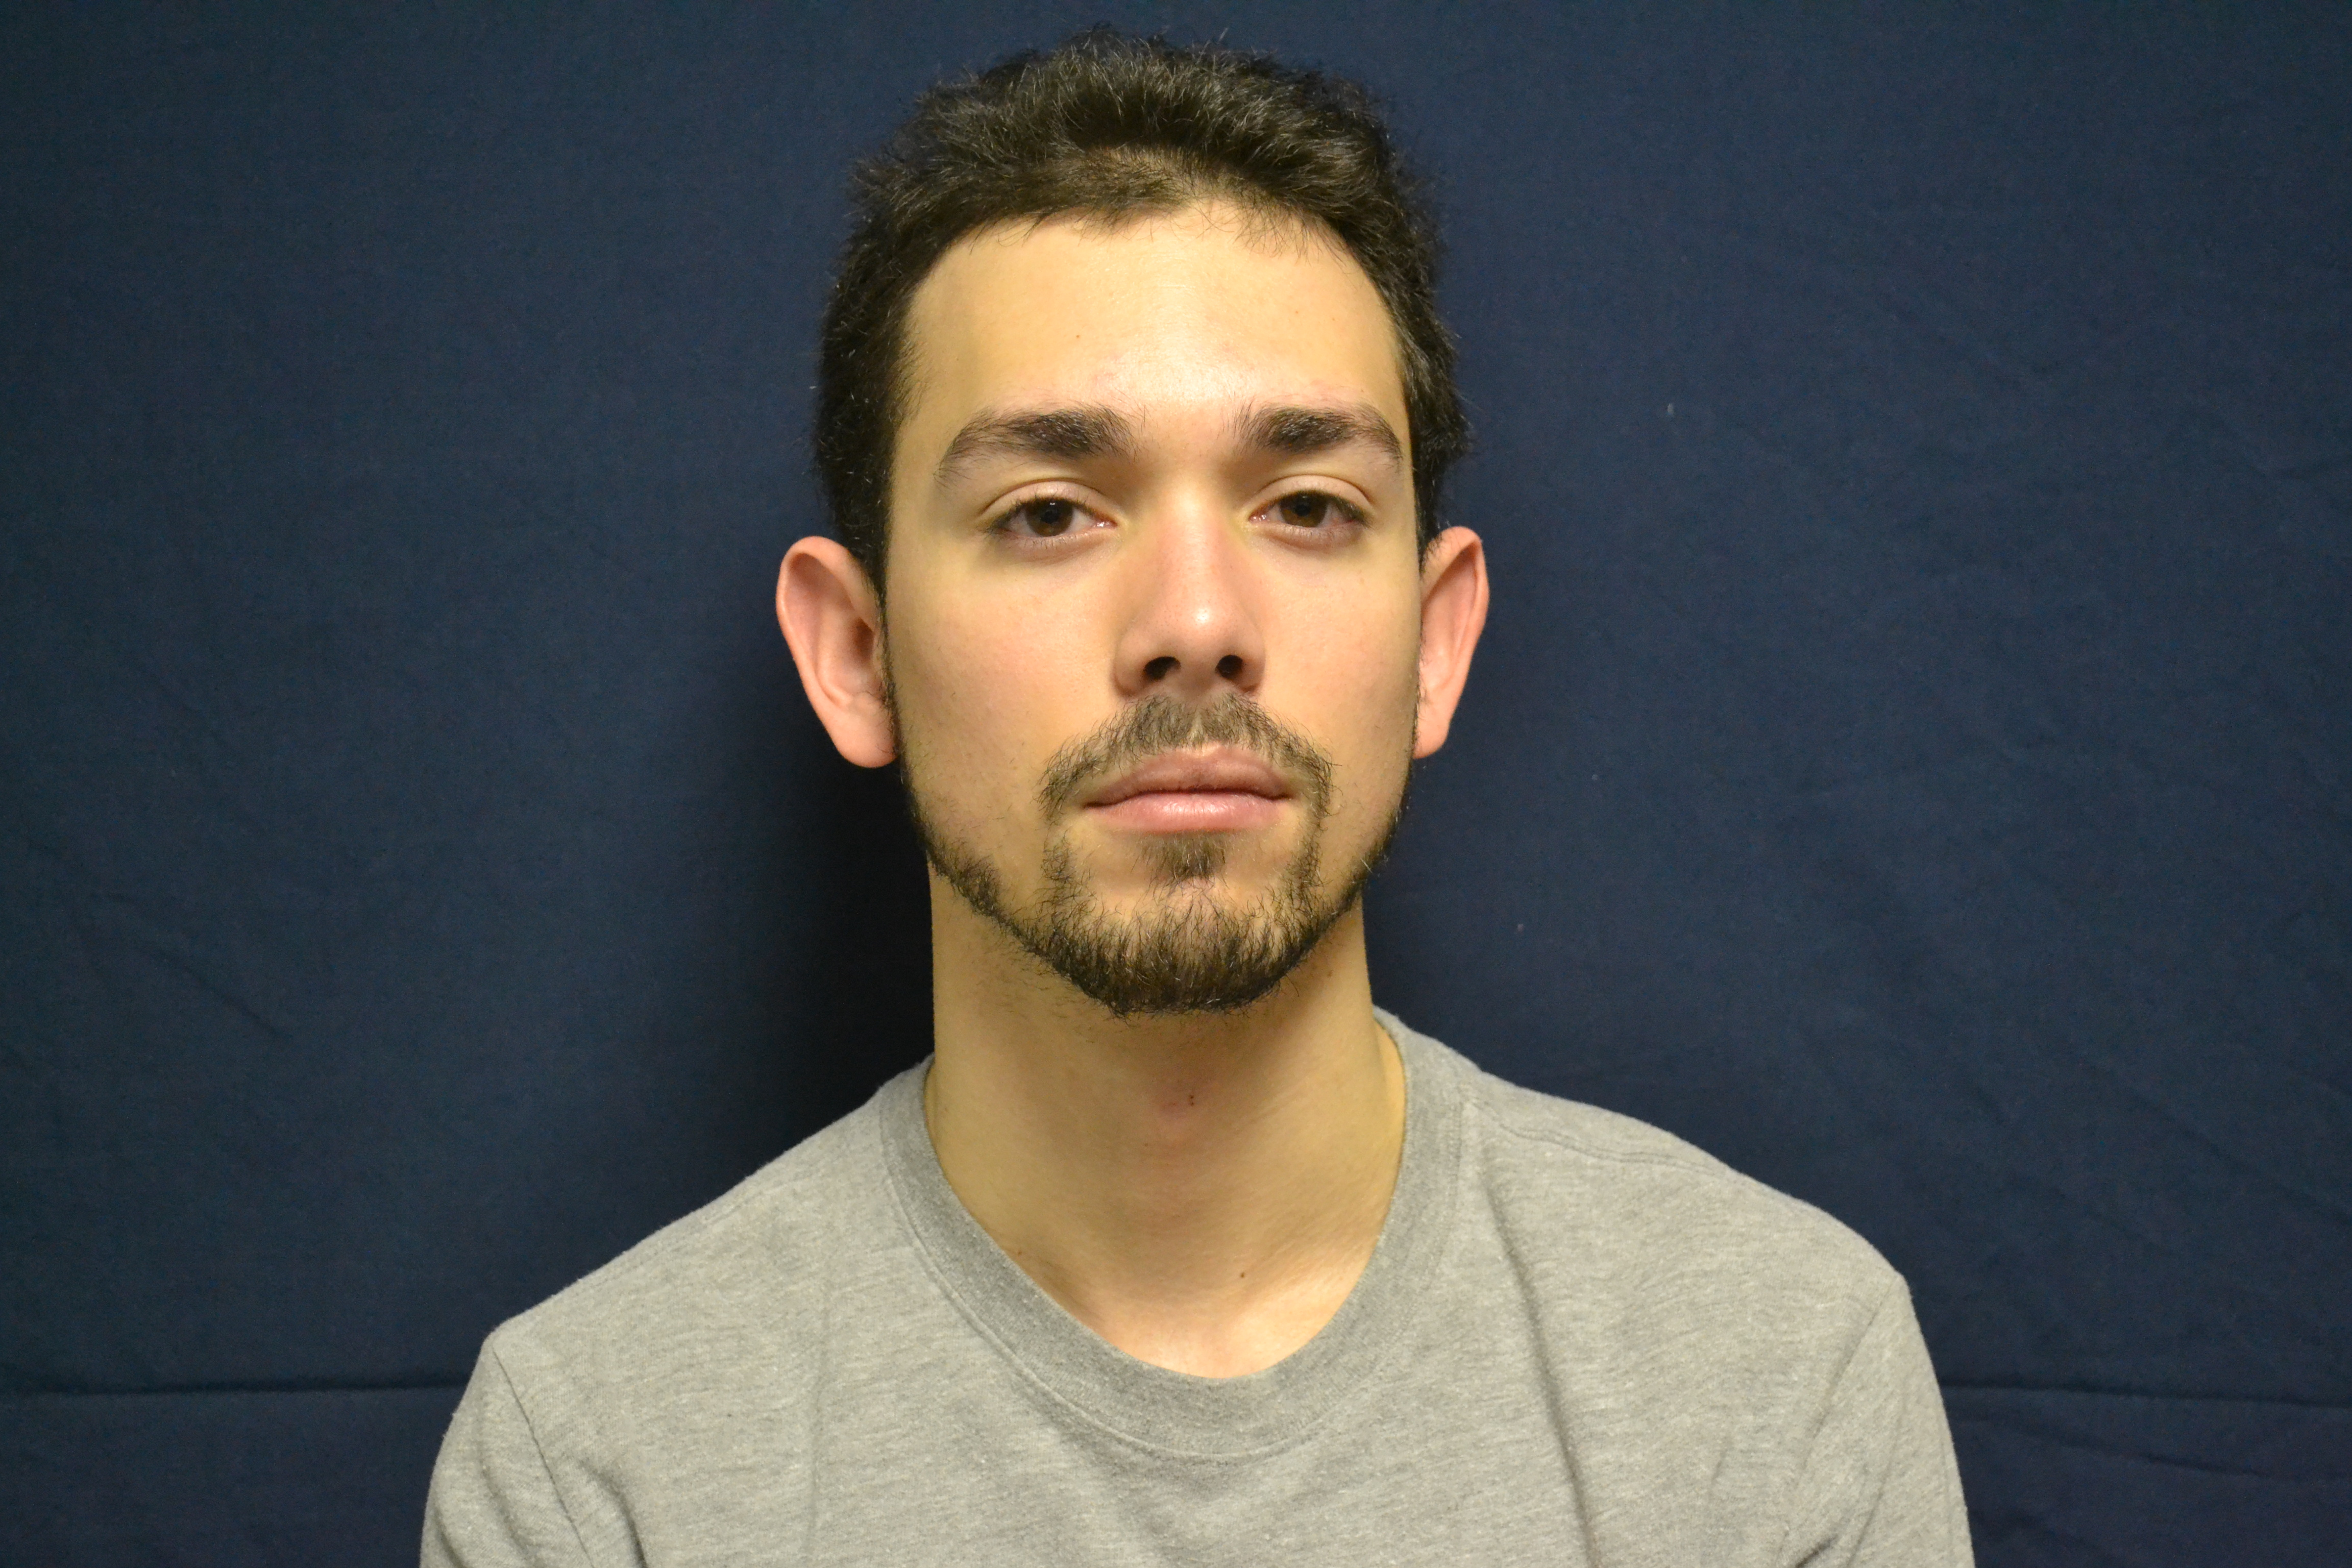
\includegraphics[scale = 0.15]{figures/ExcellentImg.jpg}
        \label{fig:excellentImg}\hspace{2cm}}
    \subfloat[Facial image with defects]
        {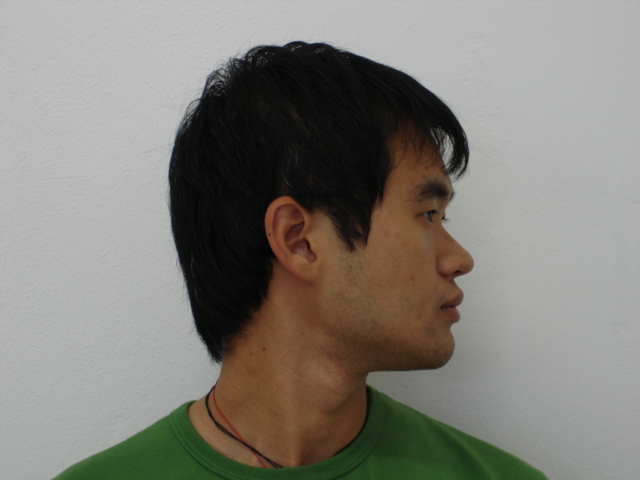
\includegraphics[scale = 0.23]{figures/FairImg.jpg}
        \label{fig:defectedImg}}
\end{figure}

Image \ref{fig:excellentImg} checks all bullet points 


\begin{figure}[H]
\centering
    \subfloat[Excellent facial image]
        {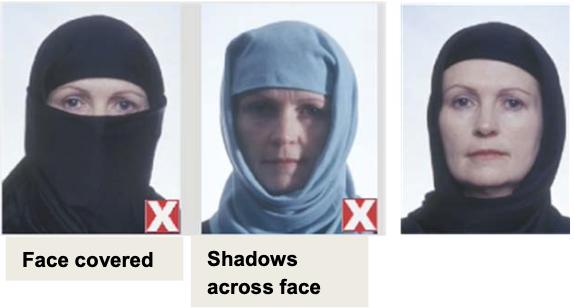
\includegraphics[scale = 0.65]{figures/FaceCovered.png}}
    \subfloat[Facial image with defects]
        {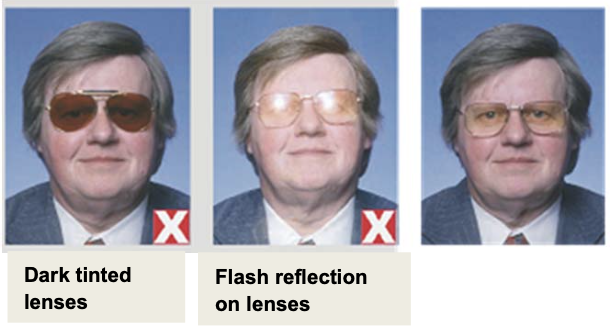
\includegraphics[scale = 0.65]{figures/SunglassesTinted.png}\hspace{3cm}}
        \vspace{0.5cm}
        \newline
    \subfloat[]
        {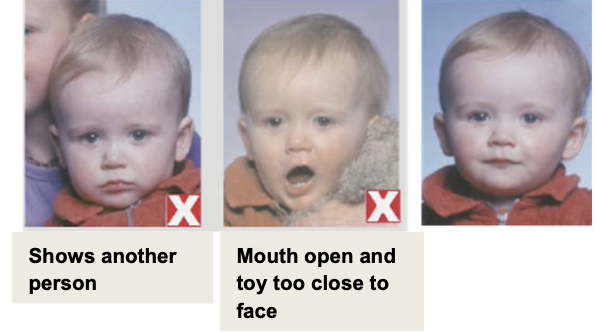
\includegraphics[scale = 0.65]{figures/BabyOpenMouth.png}}
\end{figure}


\section{Image quality metrics} 
Mobai chose the IQMs used in our application. The reason for choosing these specific metrics was their differences in terms of evaluating images of faces. 

Both metrics are open-source projects. 


\subsection{ISO metric}

\subsection{FaceQNet}